\subsection{Simplified Ikeda method}
\label{se:simplified_ikeda}
The \emph{Simplified Ikeda method} \cite{kawahara_simple_2011} has been implemented with the intention to be used both as a benchmark and maybe also as a sub-component of a new method. The examples from \cite{kawahara_simple_2011} was recalculated to check that the method has been implemented correctly.
The method has been implemented as a function where the total roll damping and its component is calcultated: 
\begin{equation} \label{eq:simplified_ikeda_equation}
\left( B_{44}, \  B_{F}, \  B_{W}, \  B_{E}, \  B_{BK}, \  B_{L}\right) = \operatorname{Ikeda_{simplified}}\left(L_{pp},beam,C_{b},A_{0},OG,\phi_{a},BK_{L},BK_{B},\omega,T,V\right)
\end{equation}


\begin{figure}[H]
    \centering
    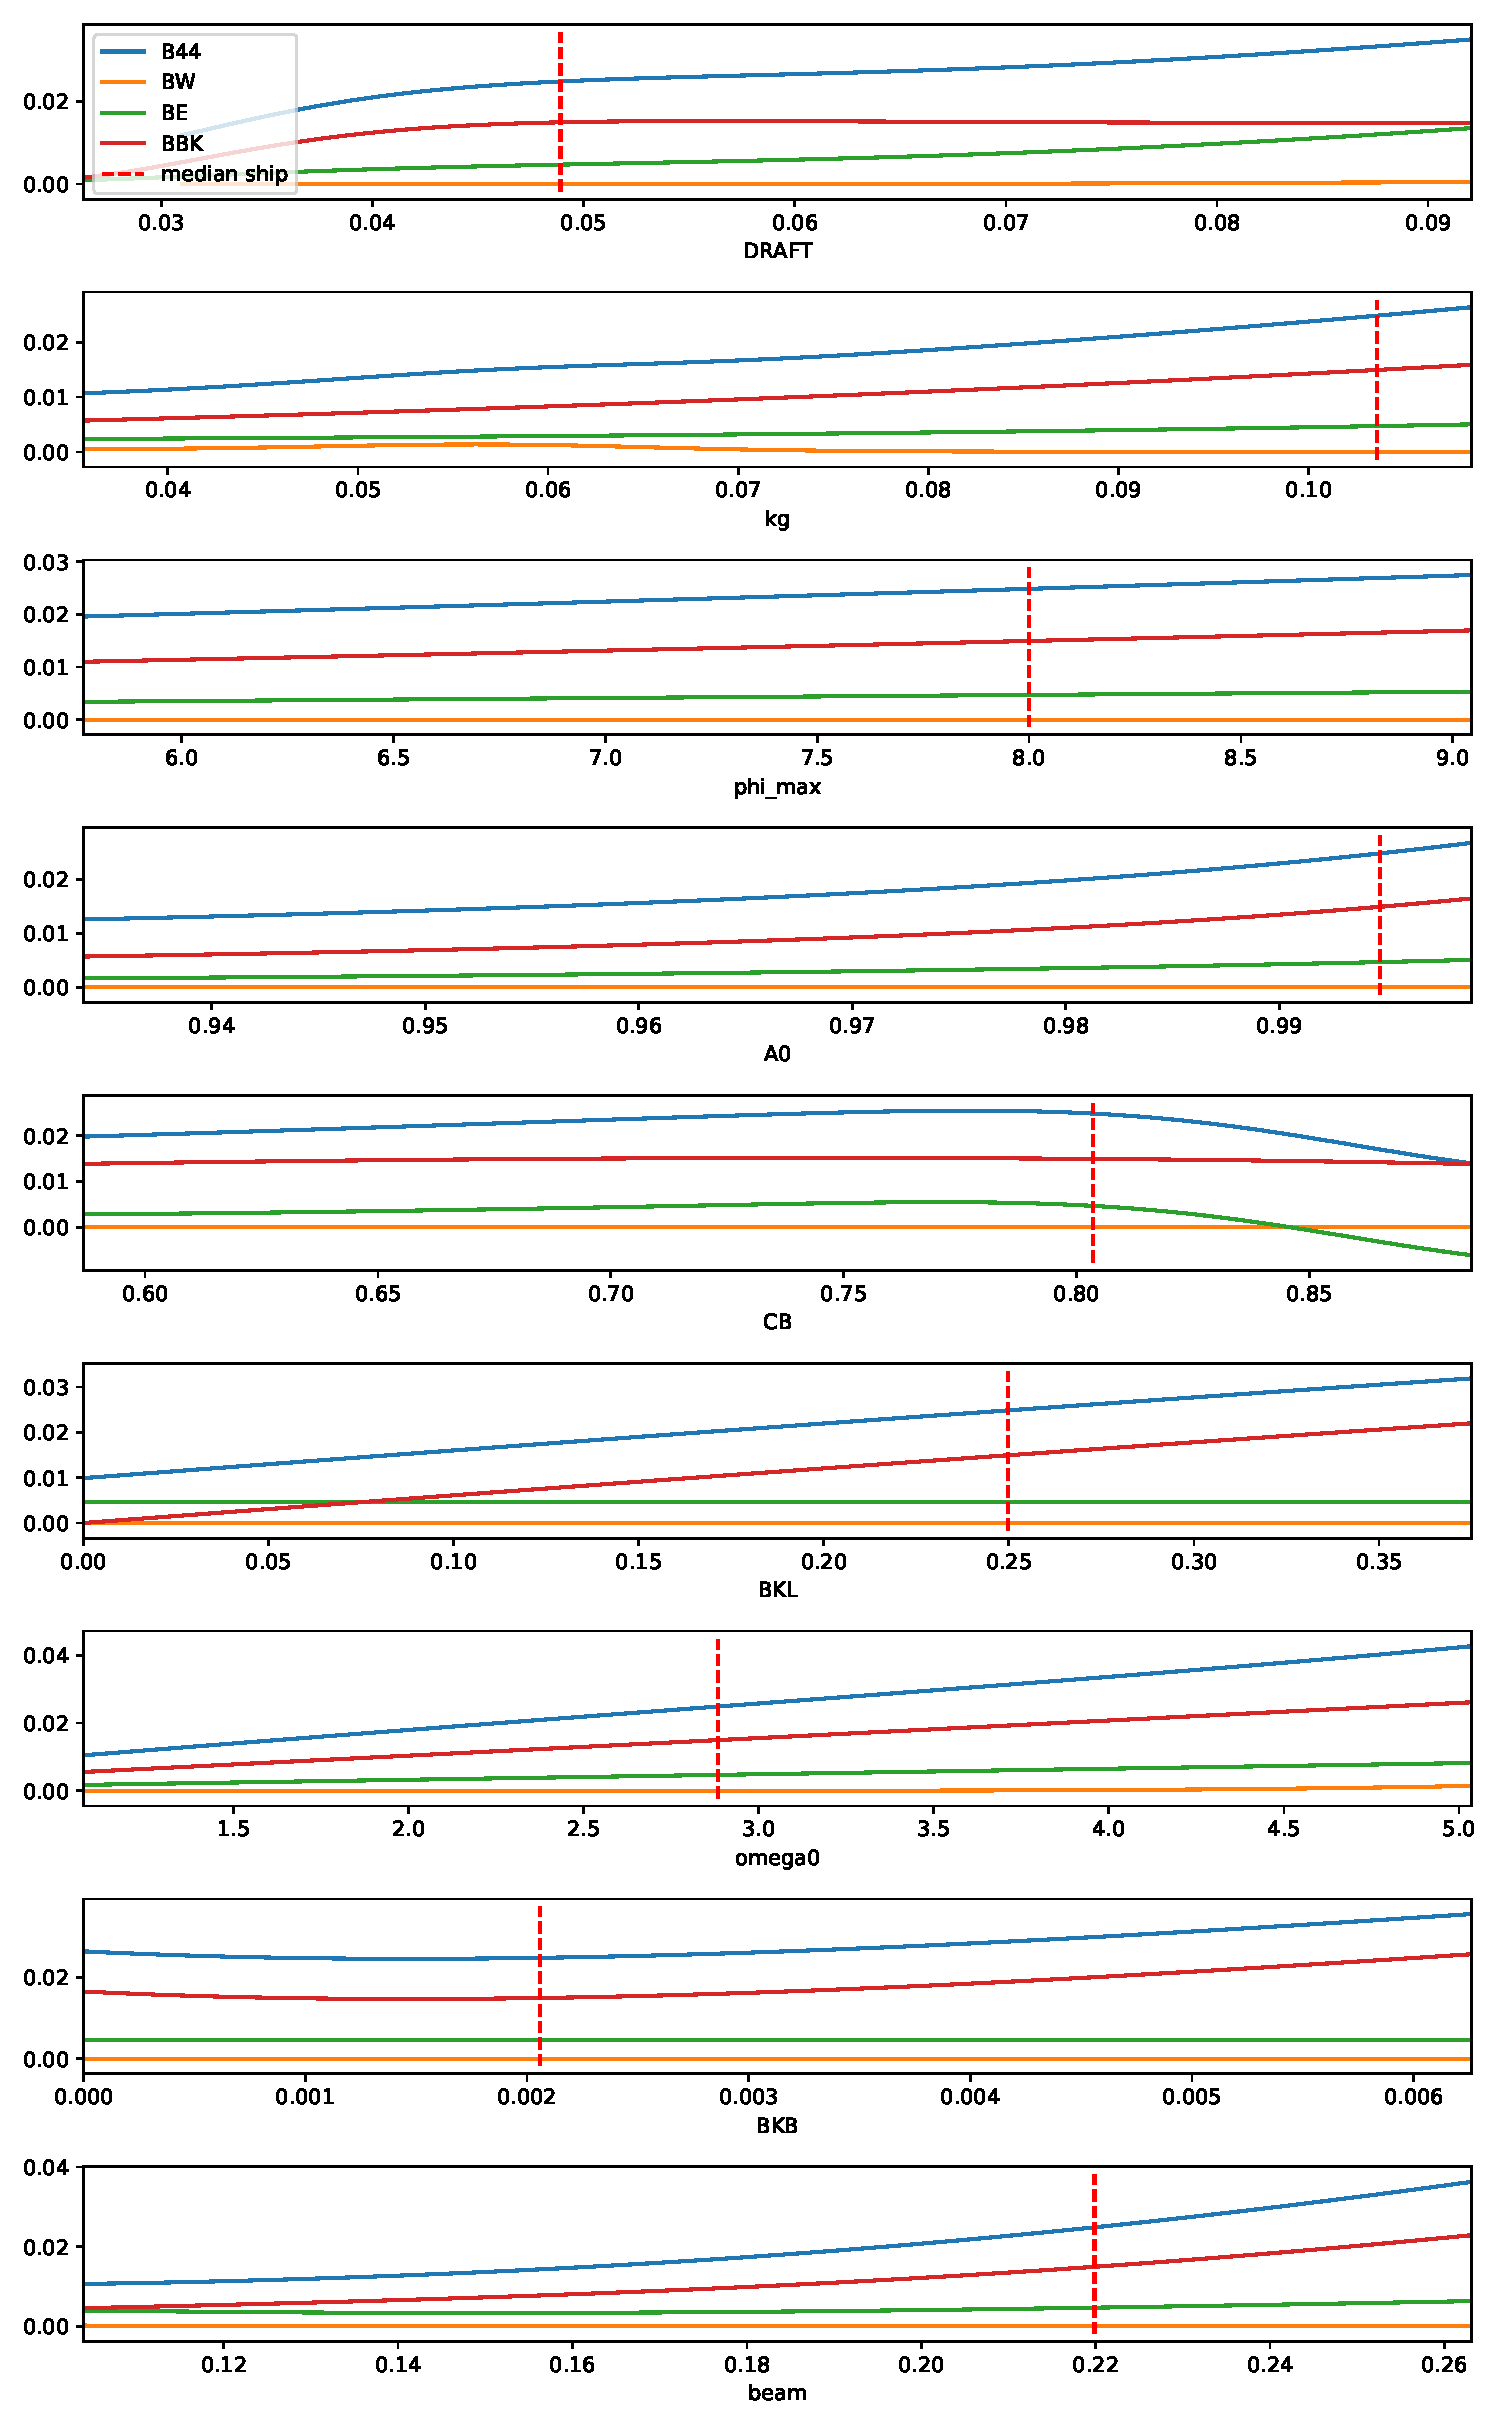
\includegraphics[width=0.9\columnwidth]{figures/ikeda_variation.pdf}
    \caption{Simplified method parameter variation}
    \label{fig:ikeda_variation}
\end{figure}

A quadratic roll damping model can be linearized using the equivalent linear damping coefficient \cite{himeno_prediction_1981}:
\begin{equation}
B_{e} = B_{1} + \frac{8 B_{2} \omega_{0} \phi_{a}}{3 \pi}
\end{equation}

In order to obtain the damping coefficients $B_1$ and $B_2$ in the quadratic model in equation \ref{eq:roll_decay_equation_himeno_quadratic} roll damping is calculated for two or more roll amplitudes ($\phi_a$). $B_1$ and $B_2$ is obtained by fitting equation \ref{eq:B_e_equation} to this data as shown in figure \ref{fig:ikeda_B_1_B2}.  

\begin{figure}[H]
    \centering
    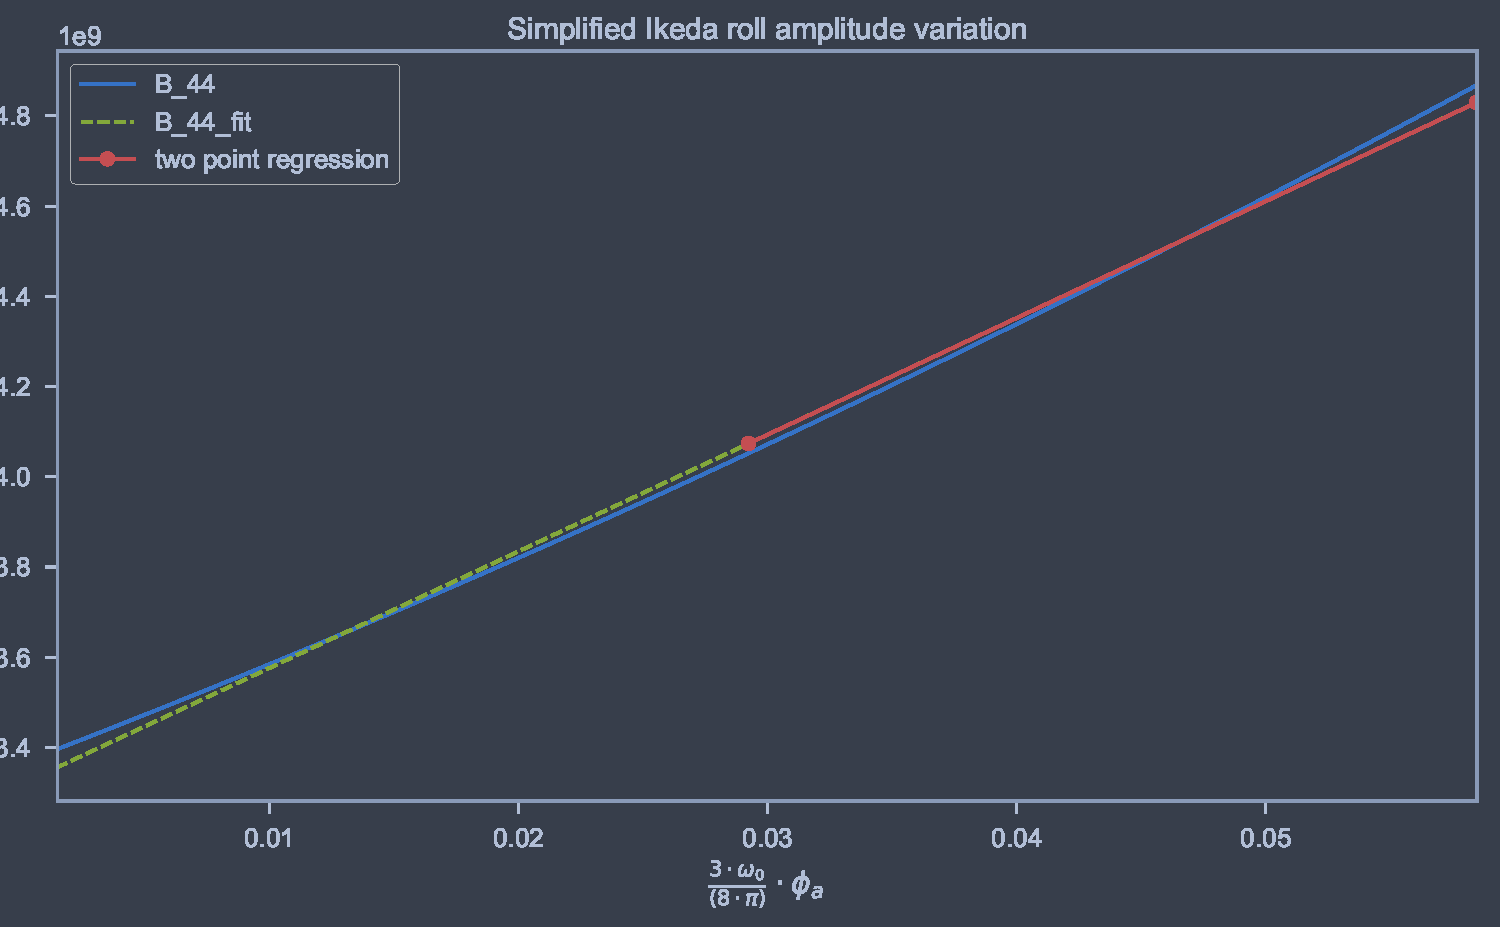
\includegraphics[width=\columnwidth]{figures/ikeda_B_1_B_2.pdf}
    \caption{Variation of roll amplitude to derive $B_1$ and $B_2$}
    \label{fig:ikeda_B_1_B2}
\end{figure}

A parameter variation was conducted in order to study the simplified method.
A "median ship" with the most usual parameters in the database was chosen as the baseline of the variation. The parameters were varied to the extreme values of the database, see figure \ref{fig:ship_parameters} for more details. 

Figure \ref{fig:ikeda_variation} shows this variation where all parameters have been none dimensionalized using froude scaling with $L_{pp}$ as scale factor. 
It seems that length to beam ratio between 0.23 and 0.24 has a huge peak. Also length to draft ratio below 0.034 has a large peak. 



\begin{figure}[h]
    \centering
    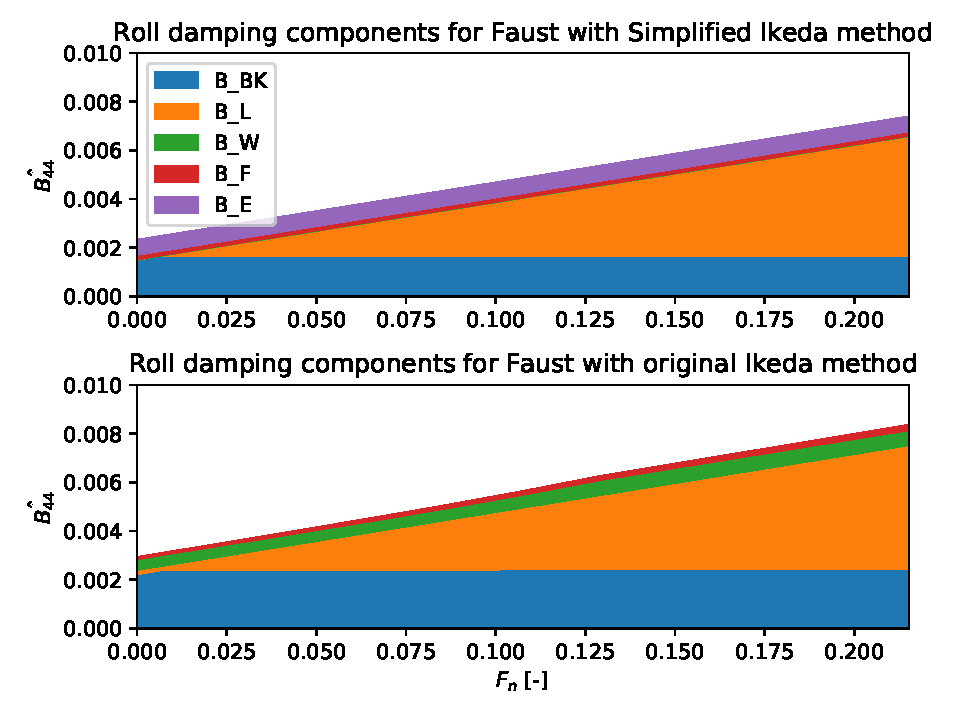
\includegraphics[width=\columnwidth]{figures/ikeda_vs_simplified.pdf}
    \caption{Roll damping components calculated with Ikeda and Simplified Ikeda for PCTC Faust}
    \label{fig:ikeda_vs_simplified}
\end{figure}







